\documentclass{article}
% \usepackage[margin=2.5cm]{geometry}
\usepackage[margin=2.5cm, headheight=0pt, headsep=1cm]{geometry}
\usepackage{enumerate, fancyhdr, graphicx, amsmath, nth}
\usepackage[binary-units=true]{siunitx}

\title{Big Brother Is Watching}
\author{Paul Chesnais (pmc85), Nimit Sohoni (nss66) and Matthew Siebert (mrs345)}
\date{\today}

\pagestyle{fancy}
\fancyhead{}
\lhead{pmc85, nss66 and mrs345}
\chead{Big Brother}
\rhead{\today}
\fancyfoot{}
\rfoot{\thepage}
\lfoot{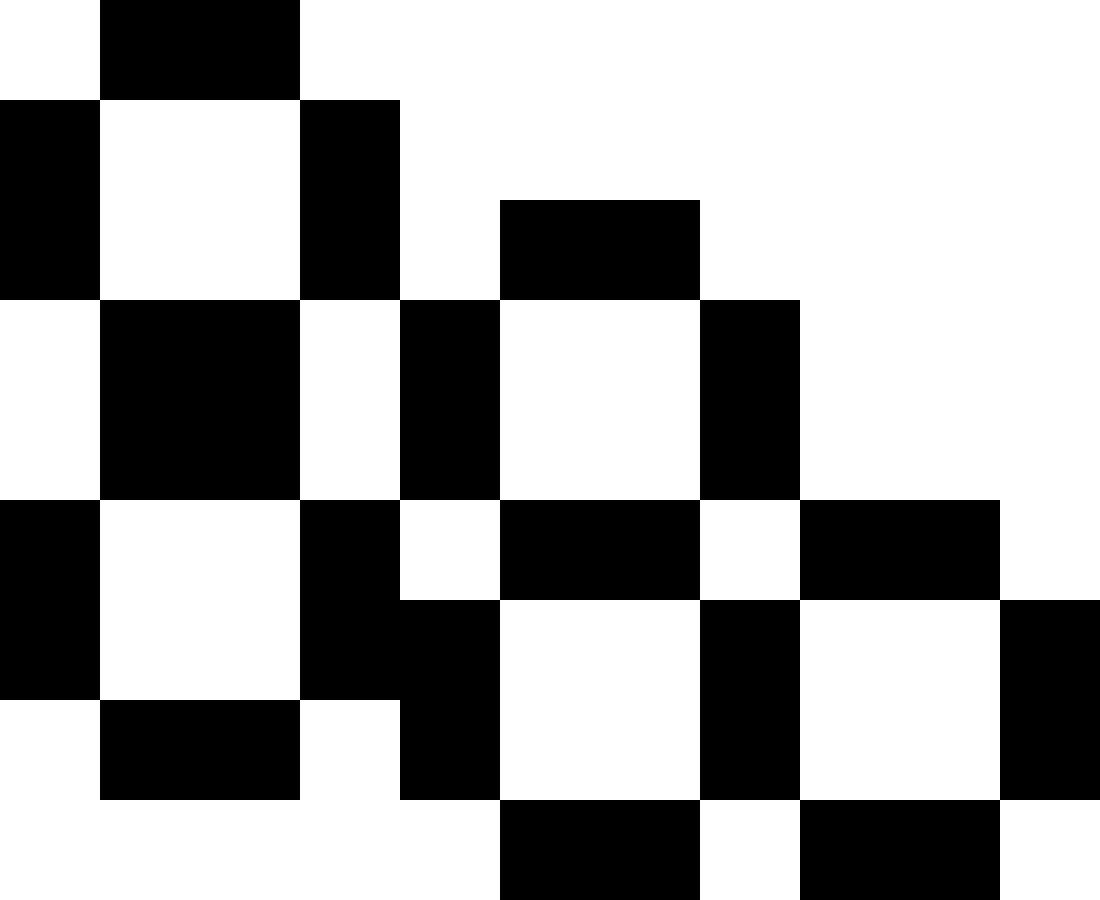
\includegraphics[height=20pt]{Logo}}
\renewcommand{\headrulewidth}{0.5pt}
\renewcommand{\footrulewidth}{0.5pt}

\DeclareSIUnit{\mph}{mph}

\usepackage{listings, color, times, textcomp, float, hyperref, subcaption}
\definecolor{mygreen}{RGB}{28,172,0} % color values Red, Green, Blue
\definecolor{mylilas}{RGB}{170,55,241}
\lstset{language=Matlab, basicstyle=\scriptsize\ttfamily,breaklines=true,
frame=single,morekeywords={matlab2tikz},keywordstyle=\color{blue},
morekeywords=[2]{1},keywordstyle=[2]{\color{black}},
identifierstyle=\color{black},stringstyle=\color{mylilas},
commentstyle=\color{mygreen},showstringspaces=false, numbers=left,
numberstyle={\tiny \color{black}},numbersep=9pt,emph=[1]{for,end,break},
emphstyle=[1]\color{red},literate={~} {\texttildelow}{1}}

\newcommand{\exo}[1]{\section*{Exercise #1}}
\newcommand{\prob}[1]{\section*{Problem #1}}
\newcommand{\quest}[1]{\section*{Question #1}}
\newcommand{\e}{&=&}
\newcommand{\p}[1]{\times 10^{#1}}

\begin{document}
\maketitle
\thispagestyle{empty}

\section{Abstract}
\label{sec:abstract}
Several models were developed to facilitate the perpetual surveillance of Gotham City using Micro unmanned Aerial Vehicles in order to catch jaywalkers. These models are optimized to handle separate scenarios involving maximum visit intervals, sharp turns requiring more energy/fuel, recharging/fueling rates, densities of jaywalkers, and the biased knowledge of the drone programmers. We represent Gotham City as rectangular grid in order to simplify our models. Our three approaches that handle these problems consist of an optimal path/contingency model that minimizes the number of turns and accounts for drone failures, a blocking model that subdivides Gotham in to smaller rectangles that individual drones traverse, and a greedy random walk model that adds a randomized effect to the drones paths.
\section{General Assumptions}
\label{sec:general_assumptions}
\paragraph{Representing Manhattan}
\label{par:representing_manhattan}
First, we want to justify our representation of Manhattan. Manhattan is a long thin strip of land, spanned vertically by \emph{avenues} and horizontally by \emph{streets}. Manhattan is effectively 250 streets long, and 10 avenues wide. A Manhattan city block is \SI{80}\m by \SI{274}\m. We can approximate Manhattan, or at least this hypothetical version of Manhattan as part of Gotham City, to be a grid 250 blocks long by 30 blocks wide, where a block is an arbitrary unit of distance, in this case \SI{80}\m. In this representation, Central Park is 10 blocks wide and 51 blocks long, since the real Central Park is 3 avenues wide and goes from \nth{59} Street to \nth{110} Street, occupying the middle 3 avenues \cite{centralpark}. Similarly, if we take Gotham University to be the fictional equivalent of Columbia University, which is found between \nth{110} Street and \nth{122} Street and spans the 3 westernmost avenues of Manhattan \cite{columbia}, then we can it to be an area 12 block long and 9 blocks wide. Finally, the Financial District is contained in the southernmost 20 streets in Manhattan \cite{financial}, hence we can make it occupy the last 20 rows in our matrix.

\paragraph{Representing Time}
\label{par:representing_time}
Next, we also justify our representation of time. Instead of modeling it as a continuous variable, it is better to model it as discrete steps in time, where drones can move a fixed distance and observe a fixed number of blocks per step. For simplicity, we will make these steps in time exactly one minute long.

\paragraph{Drone Speed}
\label{par:drone_speed}
Recent legislation has limited the speed of drones at \SI{100}\mph \cite{dronespeed}. Having drones zipping around Manhattan at \SI{100}\mph seems not only dangerous, it seems that they would not be able to gather very meaningful data. As such, for the purposes of this simulation, we made our drones relatively slow and limited the to a speed of 10 blocks per minute.

\paragraph{Drone Sight}
\label{par:drone_sight}
For this particular fictional reality, we assume that drones need to take pictures of the jaywalkers' faces in order to flag them. As such, we assume in a drone can only see jaywalkers in the intersection it is currently hovering over. This means that a drone needs to physically fly over a particular intersection for it to be counted as ``visited''.

\section{Simplifications}
There are two simplifications that we reserved the right to make when designing our strategies. They make the solutions more elegant and easier to compute, while not preventing us from then generalizing our optimal solutions back to the original problem.
\paragraph{Flight and Recharge Time}
\label{par:flight_and_recharge_time}
One parameter that was made unclear is once drones run out of fuel, how long does it take them to recharge? Suppose we have an optimal solution that requires exactly $n$ drones. If it takes a drone exactly 5 hours to recharge, and we need to keep $n$ drones in the air at all times, then we need a minimum of $2n$ drones to guarantee our ability to do so. Similarly, if the time to recharge is 1 hour, then we can interleave the drones' schedules such that one drone goes down every hour, and we only need $n+1$ drones to achieve the optimal solution. There is an inverse relationship between the amount of time it takes to recharge the drones (relative to the amount of time a drone can stay in the air), and the total number of drones needed to achieve a particular solution. As such, we can begin by finding an optimal solution requiring $n$ drones where drones can fly indefinitely, then fine tuning $n$ with regards to the flight and recharge time constraints accordingly.
\paragraph{Charging Stations}
\label{par:charging_stations}
Another consideration for this summation may be that the drones can only be launched from a limited number of charging stations. Suppose a strategy involves splitting up Manhattan into quadrants, then assigning drones for each quadrants. If drones can only launch from certain locations within Manhattan, they may take some time to get their respective areas, which may lead to lost observation time. There are two reasons why the following models do not take this into account. First of all, in the grand scheme of the strategy, what matters is what happens in the majority of the time, not the small amount of time it takes for the drone to move to its area, relative the total amount of time the drone is in the air. The other reason is that while the speed of our drones is 10 blocks per minute while watching for jaywalkers, nothing was said about their actual top speed. There is reason to believe that if a \SI{100}\mph speed limit exists, some drones are capable of reaching that speed, and will indeed do so if required while relocating to a new quadrant. Therefore we can assume that drones ``spawn'' in the correct location at the beginning of time.

% Matt's stuff n' things
\section{Optimal Path Model / Contingency Plan}
\label{sec:optimal_path_model}

The two contingencies that we must account for are the fuel penalty applied when drones make sharp turns, and the possibility that drones may be grounded for repairs. In order to ensure that every location is periodically observed without reprogramming the drones, the drones must all follow the same path and be equally spaced. The path that accomplishes this and minimizes the total number of turns is similar to the one shown in Figure \ref{path}.
\begin{figure}[htb!]
    \centering{{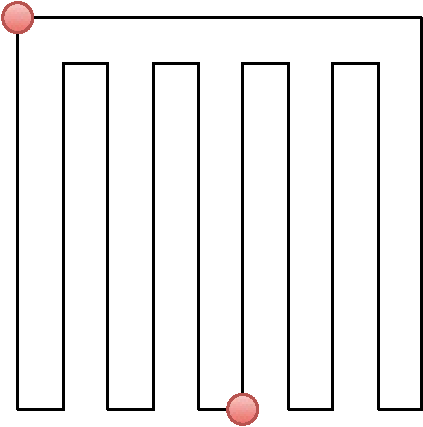
\includegraphics[width=7cm]{figures/optimal_path.pdf} }}
    \caption{The shape of the path with the minimum number of turns that visits every area of the city.}
    \label{path}
\end{figure}
\newline In our case Manhattan is modeled as being $30\times 250$ blocks. The similar path for this layout has 60 turns and a total path length of 7500 blocks ($\sim 250$ miles). If the speed of each drone is 30 mph then each drone can fly 3000 blocks before having to refuel if we do not account for turning penalties. Since we were not given a specific parameter for drone refueling rates, need to create a flexible model that describes the refueling rates effects on the number of drones required.
\begin{eqnarray}
N \geq \frac{R n_{c}}{T}\label{backup drones}
\end{eqnarray}
Equation \ref{backup drones} describes the number of extra drones needed ($N$) as a function of the refueling time $R$ ($n_{c}$ and $T$ are the number of currently deployed drones and their fuel capacity in hours respectively). We can see from this equation that if the refueling time equals the length of time for which drones can fly, then $N = n_{c}$.  So we would need a total of $2n_{c}$ drones as expected.
This means that in the worst case we need to have an additional supply of available drones equal to the number of operating drones that can be deployed when fuel is depleted. This also assumes that refueling the drones takes less than 5 hours.
\newline If the drones are equally spaced, then the distance between them in blocks is simply $L/n_{c}$ where $L$ is the total path length (7500 blocks). By setting the maximum time interval $t$ to 15 min in Equation \ref{max time interval} we can solve for the minimum number of drones required given that the drones travel at a rate $R = 10$ blocks/minute (30mph). Our representation of the city requires $n_{c} = 50$ for a maximum unobserved interval of 15 minutes.
\begin{eqnarray}
t = \frac{L}{n_{c}R} \label{max time interval}
\end{eqnarray}
\newline Now we account for the possibility that drones can break down and be grounded for repairs. We analyze the effect of at most 30\% becoming unusable. We assume that if a drone fails then the currently operating drones spread out evenly over the entire path to keep visit intervals at a minimum. Figure \ref{failed} shows the maximum unobserved time interval given drone failings ranging from 0 to 30\%. If 30\% fail then the maximum interval is increased to 21.12 minutes.
\begin{figure}[htb!]
    \centering{{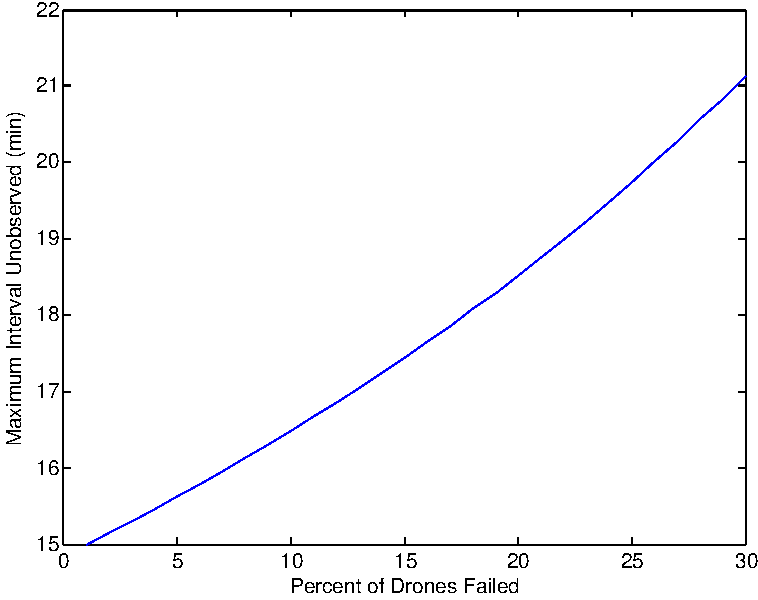
\includegraphics[width=7cm]{figures/failed_drones-crop.pdf} }}
    \caption{Drone failure effects on maximum visit interval}
   \label{failed}
\end{figure}
If it is extremely important to keep the interval at 15 minutes, then the city will need to keep extra reserve drones to deploy when drones need repair. This number would be equal to $.3n_{c} = 15$ backup drones.
\begin{eqnarray}
Total MAVs = Deployed + Backup Fuel + Backup Repair \label{totaldrones}
\end{eqnarray}
If this plan is implemented then the total number of drones that the city needs to adequately observe all areas is described by Equation \ref{totaldrones}. The worst case would be if refuel times were long and it was mandatory to keep all visit intervals within 15 min. This would require 50 drones to be deployed at all times, 50 should be readily available to deploy when operating drones run out of fuel, and 15 should be readily available to replace any broken drones. This gives us a total of 115 drones. This solution yields a density of 6.13 drones per square mile. The best case scenario would take the refuel times to be negligible and a more flexible tolerance for maximum visit intervals. This case would not require any backup drones for refueling or failures and the resulting an optimal value of 50 total drones (2.67 drones per square mile). The true solution will therefore lie in the range of 50 - 115 drones and depend on the real constraints of the situation subject to the methods we have developed.

% Nimit's stuff and things
\section{Block Model}
\label{sec:block_model}
The block model assumes that an approximation to the optimal number of drones can be achieved by splitting up Manhattan into non-overlapping rectangular blocks, each of which is assigned a drone to cover that area. The rectangles must therefore be small enough so that the drones can cover them in 15 minutes. Our algorithm iterates through all pairs of rectangle dimensions that are small enough for a single drone to cover in 15 minutes, and tiles Manhattan with these rectangles. If the dimension of Manhattan is not divisible by the rectangle dimension, we take the "leftover" area that is not covered by any rectangle and pass that area back into a recursive call to the algorithm (it may be tiled with different-sized rectangles). Finally, we select the tiling arrangement that covers Manhattan with the least number of blocks, and therefore the fewest drones.

To do this, we first need to determine how long it takes for a single drone to survey a rectangular block of dimension m by n. However, we also note that for the drone to survey a collection of points every $x$ minutes, it is not enough to simply visit all of the points within $x$ minutes, it must also \textit{return to the starting point} within $x$ minutes, otherwise the starting point will go more than $x$ minutes without being visited.

To simplify things, select some time step such that the drone can survey exactly one grid point per time step. Then, if either $m$ or $n$ is even, the amount of time it takes is just $m*n$. Proof: See Figure \ref{path} in section 4, and note that the number of "zigzags" is even and the path does not cross over itself. However, if neither is even, we may not be able to traverse the rectangle and return to the starting position in $m*n$ steps. Instead, we can traverse the rectangle in a similar zigzag pattern (with the long edge of the zigzags perpendicular to the longer edge of the rectangle), and then at the end of the last zigzag (which will end in the middle of the rectangle instead of at the starting corner), move towards the starting corner, which will take $min(m,n) - 1$ time (see Figure \ref{path2}). The exception to both cases is if either $m$ or $n$ is 1. Assume WLOG that $m = 1$; in this case, it will take $2n - 1$ time to traverse all the grid points and return to the starting position, since once we traverse all the grid points (say, from "left to right"), which takes $n - 1$ steps, we will have to retrace our steps, which takes $n-1$ more steps.

\begin{figure}[htb!]
    \centering{{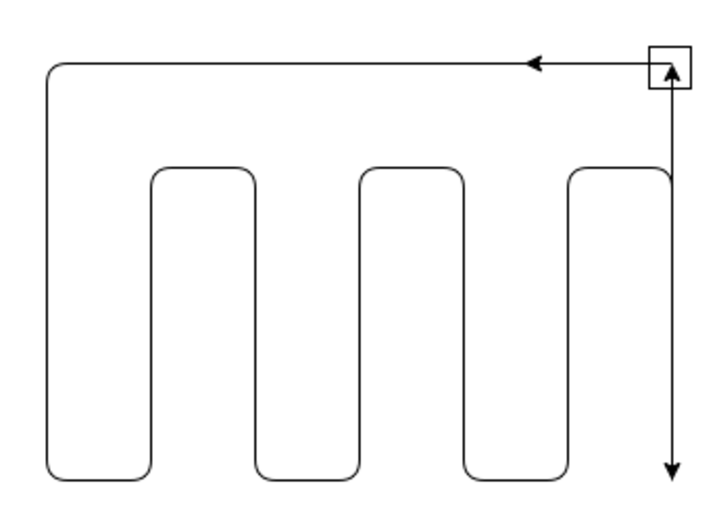
\includegraphics[width=7cm]{figures/odd_path.pdf} }}
    \caption{The shape of a path in a rectangle with an odd height and odd width. The path begins in the top right corner and goes to the left, and reverses directions from downward to upward when it gets to the bottom right corner.}
    \label{path2}
\end{figure}

Using this formula, we are ready to find the optimal arrangement of rectangular blocks that covers Manhattan while using the fewest drones.

For example, when we model Manhattan as a 30 by 250 grid, and if we assume that each drone can survey one grid point per minute, then the algorithm tells us that the "main" tiling will be 7 by 2 blocks. So, a contiguous 28 by 250 area (without loss of generality, we can assume it is in the upper left corner) will be covered with a 4 by 125 tiling of rectangular blocks. Then, there is a 2 by 250 area remaining. This area will be tiled with 35 2 by 7 blocks. Finally, there will be a 2 by 5 block left over. This block is small enough for one drone to survey in one minute. Therefore, the total number of blocks is $4*125 + 35 + 1 = 500 + 36 = 536$ blocks, and so 536 drones.

If we assume each drone can survey ten grid points per minute, then we get that the main tiling will be a 10 by 5 tiling of 3 by 50 blocks. There is no space left over (every grid point is covered by some block), so the total number of drones is just 50.

This method can be extended to the case where some areas must be observed more often than others. We can just assume that these areas are rectangular (which is a fairly good assumption in this case) and treat these areas as separate blocks.

% Paul's stuff n' things
\section{Greedy Random Walk}
\label{sec:greedy_random_walk_model}
Since some fellow jaywalkers don't want us to have an advantage when walking the in the streets of Manhattan, we also need a strategy that is a little more unpredictable. Part of the problem with the strategies outlined above is that knowing the location of a single drone lets someone with inside knowledge about the strategy infer the location of every other drone, or at least the location of neighboring drones. One response to this complaint would be to make the drones travel a more random path. The following strategy does just that, and works even when areas of Manhattan have different densities of jaywalkers.

\subsection{Global State}
\label{sub:global_state}
One of the requirements of this strategy is that a global state accessible by all drones is required. It seems reasonable to assume that cellphone networks still exist in 2084, and therefore that all of our drones are connected to the Internet. Two pieces of information need to be kept about each node in the grid: the time at which the node was last visited, and the required frequency at which it needs to be watched.

\subsection{Greedy walk}
\label{sub:greedy_walk}
As mentioned above, drones have access to the timestamp of the last visit for a given intersection, and the amount of time that can pass before said intersection needs to be watched again. As such, the ``urgency'' or how soon a given node must be visited, can be inferred. A naive, greedy drone can therefore move to the neighboring node with the highest urgency rating, and choosing randomly between neighbors when some nodes are tied. This means that a drone’s movement is unpredictable, and seeing a drone above one intersection does not let a municipal employee infer the location of the rest of drones.

\subsection{Performance}
\label{sub:greey_performance}
This strategy can tackle both density requirements. Figure~\ref{fig:greedy_performance} show the performance of this strategy when the jaywalker density is uniform and when it is not, respectively. The vertical axis represents the mean number of nodes left unwatched for too long per moment in time over 10 simulations, and the horizontal axis represents the number of drones in flight during the simulations. There is a slight difference between Figure~\ref{fig:random_uniform} and Figure~\ref{fig:random_nonuniform} in that when the jaywalker density isn't uniform, more drones are required. This is most likely due to the fact that Gotham University and the Financial District need to be watched so often that any strategy would require more drones. This strategy manages to appropriately cover 90\% of Manhattan with 70 drones and 75 drones when the jaywalker density is uniform and nonuniform respectively, and 97.5\% of Manhattan with 90 and 95 drones respectively. One could keep adding arbitrarily many drones, but with diminishing results.

\begin{figure}[H]
\center
\begin{subfigure}[b]{0.5\textwidth}
  \center
  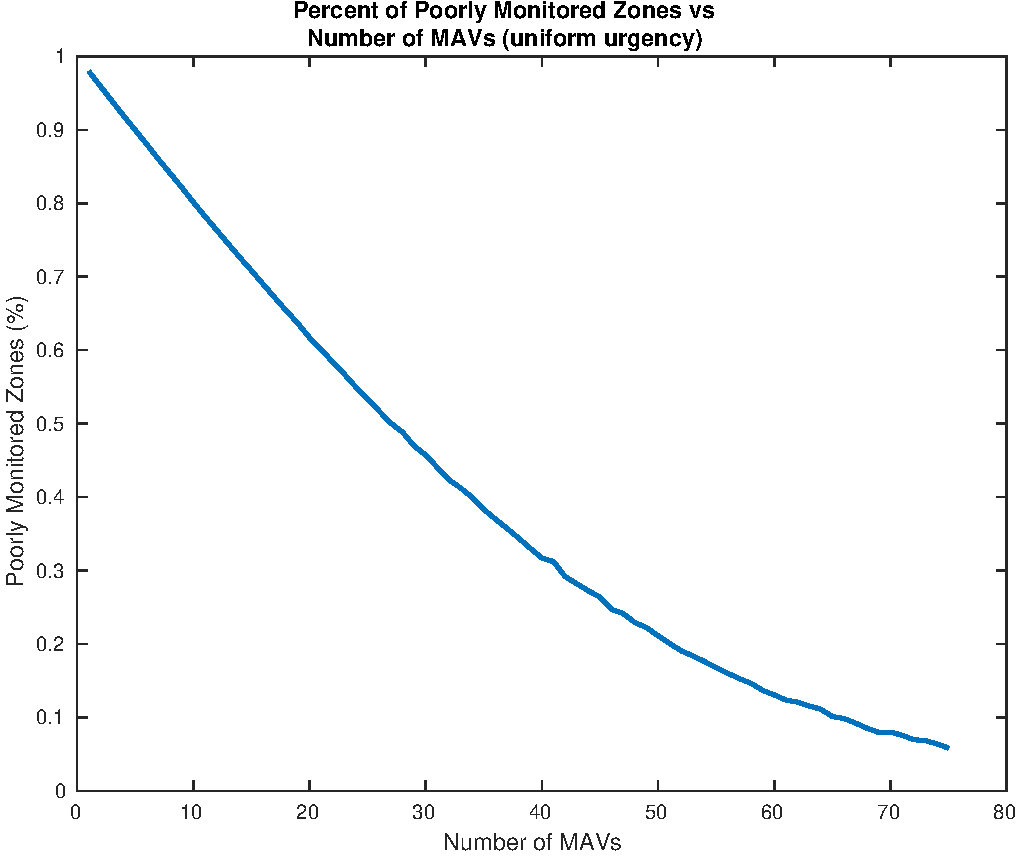
\includegraphics[width=\textwidth]{figures/random_walk_part1-crop.pdf}
  \caption{Uniform jaywalker density}
  \label{fig:random_uniform}
\end{subfigure}~
\begin{subfigure}[b]{0.5\textwidth}
  \center
  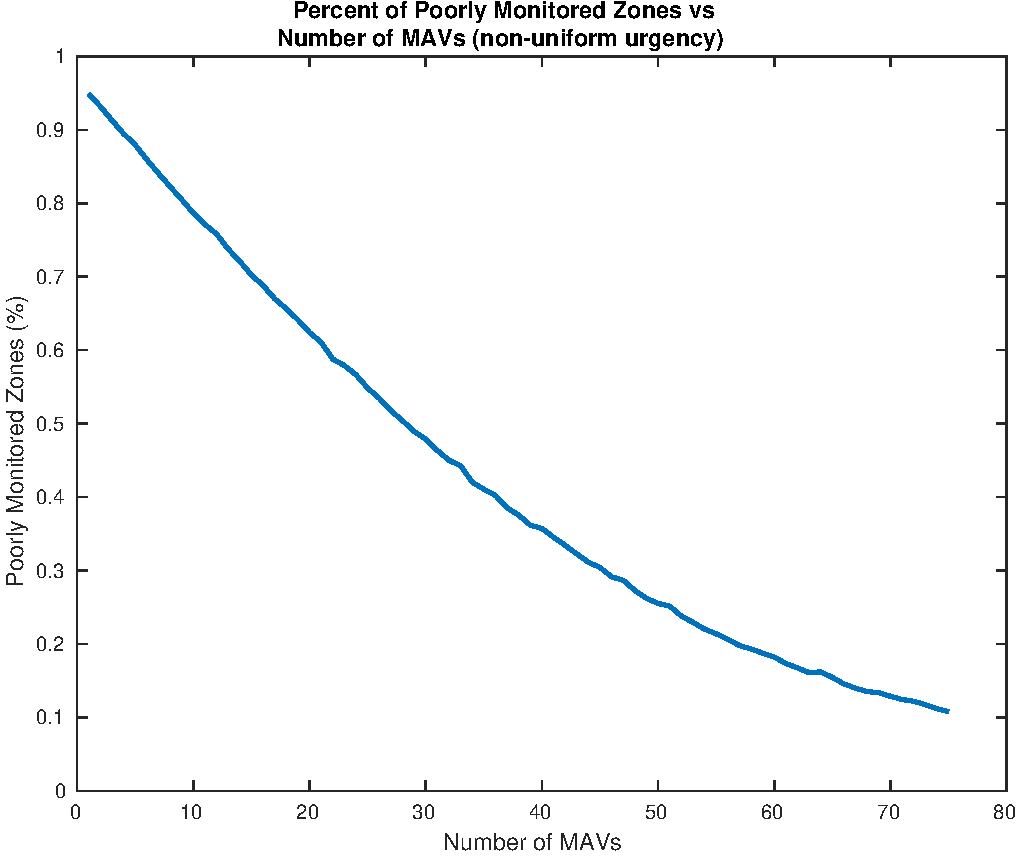
\includegraphics[width=\textwidth]{figures/random_walk_part3-crop.pdf}
  \caption{Nonuniform jaywalker density}
  \label{fig:random_nonuniform}
\end{subfigure}
\caption{Performance of Greedy Random Walk}
\label{fig:greedy_performance}
\end{figure}

\section{Conclusion}
\label{sec:conclusion}
In conclusion, it seems that one would need at least 50 drones to optimally cover Manhattan/Gotham City. Unfortunately, those drones have infinite fuel, therefore the true solution needs to be adjusted according to the ratio of the drones' flight time and their recharge time.


\section{Appendix}
\label{sec:appendix}

\subsection{Greedy Walk Source}
\label{sub:greedy_walk_source}
\lstinputlisting{models/random_movement.m}
\lstinputlisting{models/MAV.m}

\subsection{Contingency Source}
\label{sub:contingency_source}
\lstinputlisting{models/drone_failures.m}

\begin{thebibliography}{9}
  \bibitem{columbia}
    \url{https://www.google.com/maps/place/columbia+university/@40.8075355,-73.9625727,15z/data=!4m2!3m1!1s0x0:0x577933f947e52750?sa=X&ved=0CIcBEPwSMBdqFQoTCMay2Oi09cgCFQJ4Jgod360LJA}
  \bibitem{financial}
    \url{https://www.google.com/maps/place/Financial+District,+New+York,+NY/data=!4m2!3m1!1s0x89c25a18338ac807:0x2bac148b119ab3?sa=X&ved=0CIUBEPIBMA1qFQoTCKr37smw9cgCFUJkJgodYywMtA}
  \bibitem{centralpark}
    \url{https://www.google.com/maps/place/Central+Park,+New+York,+NY/@40.7828647,-73.9653551,15z/data=!4m2!3m1!1s0x89c2589a010bc7f5:0xc159962ffd2019b6}
  \bibitem{dronespeed}
    \url{http://www.npr.org/sections/thetwo-way/2015/02/15/386464188/commercial-drone-rules-to-limit-their-speed-and-altitude}
\end{thebibliography}


\end{document}